\section{Evaluation}

How we tested our solution
\begin{itemize}
    \item Performance metrics
    \item Performance parameters
    \item Experimental design
\end{itemize}

How our solution performed, how its performance compared to that of other solutions mentioned in related work, and how these results show that our solution is effective
\begin{itemize}
    \item Presentation and Interpretation
    \item Why, how, and to what degree our solution is better
    \item Why the reader should be impressed with our solution
    \item Comments
    \item Here is a cross reference to Table~\ref{tab:my_label} and Fig.~\ref{fig:my_label}.
\end{itemize}

Context and limitations of our solution as required for summation
\begin{itemize}
    \item What the results do and do not say
\end{itemize}

\begin{table}[t!]
    \centering
    \begin{tabular}{c c c}
        Problem Size (N) & Ideal runtime (sec) & Actual runtime (sec) \\
        \hline 
        1 & 1 & 1 \\
        2 & 0.5 & 0.75 \\
        4 & 0.25 & 0.56 \\
        8 & 0.12 & 0.42 \\
        16 & 0.06 & 0.31 
    \end{tabular}
    \caption{Comparison of actual and ideal runtimes for different problem sizes. The actual runtime does not equal ideal runtime in this configuration.}
    \label{tab:my_label}
\end{table}

\begin{figure}
    \centering
    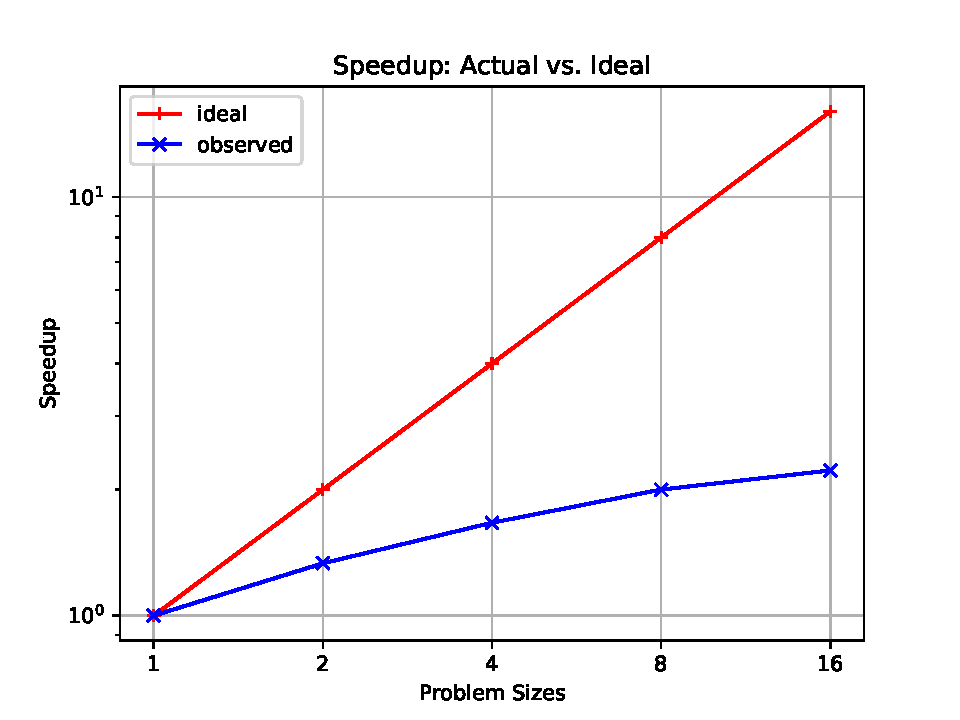
\includegraphics[width=0.45\textwidth]{Figure_1.pdf}
    \caption{Comparison of actual vs. ideal speedup with increasing problem sizes. In this case, we see the observed speedup is quite different than the ideal speedup. Try changing the vertical axis to log-scaling in the Python script that generates the chart. This figure was produced by the sample \texttt{plot\_speedup.py} file.}
    \label{fig:my_label}
\end{figure}

